\documentclass[lettersize,journal]{IEEEtran}
\usepackage{amsmath,amsfonts}
\usepackage{algorithmic}
\usepackage{algorithm}
\usepackage{array}
\usepackage[caption=false,font=normalsize,labelfont=sf,textfont=sf]{subfig}
\usepackage{textcomp}
\usepackage{stfloats}
%\usepackage{url}
\usepackage{verbatim}
\usepackage{graphicx}
\usepackage{cite}

\usepackage[breaklinks]{hyperref}
\usepackage{url}
\usepackage{breakurl}
\usepackage[normalem]{ulem}
\usepackage[para]{footmisc}
%\usepackage{hyperref}
%\hypersetup{breaklinks=true} % set automatically by hyperref?
\hyphenation{op-tical net-works semi-conduc-tor IEEE-Xplore}

%IEEE TRANSACTIONS ON AUTOMATION SCIENCE AND ENGINEERING

%https://tex.stackexchange.com/questions/479374/does-the-hyperref-breaklinks-option-have-any-effect
  \expandafter\def\expandafter\UrlBreaks\expandafter{\UrlBreaks%  save the current one
	\do\a\do\b\do\c\do\d\do\e\do\f\do\g\do\h\do\i\do\j%
	\do\k\do\l\do\m\do\n\do\o\do\p\do\q\do\r\do\s\do\t%
	\do\u\do\v\do\w\do\x\do\y\do\z\do\A\do\B\do\C\do\D%
	\do\E\do\F\do\G\do\H\do\I\do\J\do\K\do\L\do\M\do\N%
	\do\O\do\P\do\Q\do\R\do\S\do\T\do\U\do\V\do\W\do\X%
	\do\Y\do\Z\do\/\do-}

\begin{document}

%\title{A Sample Article Using IEEEtran.cls\\ for IEEE Journals and Transactions}
\title{Soft Gripper: On Specifying for Trustworthiness}
%TODO: Consider using different word instead of trustworthy as this is not well defined.

\author{Author1\_Name, Author2\_Name, ...AuthorN\_Name,
	\thanks{Author1 and Author2 are with the Department of Dep1\_Name (email: , )}
	\thanks{AuthorN is with the Department of Dep2\_Name (email: )}}
%\thanks{Manuscript received April 19, 2021; revised August 16, 2021.}}
% The paper headers
\markboth{Journal of \LaTeX\ Class Files,~Vol.~14, No.~8, August~2021}%
{Shell \MakeLowercase{\textit{et al.}}: A Sample Article Using IEEEtran.cls for IEEE Journals}

%\author{IEEE Publication Technology,~\IEEEmembership{Staff,~IEEE,}
        % <-this % stops a space
%\thanks{This paper was produced by the IEEE Publication Technology Group. They are in Piscataway, NJ.}% <-this % stops a space
%\thanks{Manuscript received April 19, 2021; revised August 16, 2021.}}

% The paper headers
%\markboth{Journal of \LaTeX\ Class Files,~Vol.~14, No.~8, August~2021}%
%{Shell \MakeLowercase{\textit{et al.}}: A Sample Article Using IEEEtran.cls for IEEE Journals}

%\IEEEpubid{0000--0000/00\$00.00~\copyright~2021 IEEE}
% Remember, if you use this you must call \IEEEpubidadjcol in the second
% column for its text to clear the IEEEpubid mark.

\maketitle

\begin{abstract}
Soft robotics is an emerging technology in which engineers create flexible devices for use in a variety of applications. %, such as surgery, prosthetics, space exploration, and grocery picking. 
Soft gripping is considered to be the most mature area in soft robotics. 
In order to advance the wide adoption of soft robots, ensuring their trustworthiness is essential.  % to advance the wide adoption of soft robots. 
There are a number of techniques for demonstrating the trustworthiness and common to all these techniques is the need to formulate \emph{specifications}, which so far has received very little attention by the soft robotics community.
The main contribution of this article is an extensive specification for the trustworthiness of a soft gripper that covers both functional and non-functional requirements, such as reliability, safety, adaptability, predictability, ethics, and regulations.  
We also highlight the need to promote \emph{verifiability} as a first-class objective in the design of a soft gripper. 
We explore our study using a case study of pick-and-place tasks of grocery items involving a recycled soft gripper.
\end{abstract}

\begin{IEEEkeywords}
	Specification, trust, soft gripper, verifiability, evolving functionality, autonomous systems, soft robotics.
\end{IEEEkeywords}

\section{Introduction}\label{introduction}
Soft robotics is an emerging technology in which engineers create flexible devices for use in a variety of applications, such as surgery, prosthetics, space exploration, and grocery picking. 
Soft gripping is considered to be the most mature area in soft robotics. 
In order to advance the wide adoption of soft robots, ensuring their trustworthiness is essential. 
\emph{Trust} may vary, as it can be gained and lost over time, and different research disciplines define trust in different ways. 
Autonomous systems (ASs) (e.g. soft robotic systems) are considered \emph{trustworthy} when the design, engineering, and operation of these systems generate positive outcomes and mitigate outcomes which can be harmful~\cite{Naiseh2022}.
Trustworthiness can be dependent on many factors such as: (i) explainability, accountability, and understandability to different users; (ii) robustness in dynamic and uncertain environments; (iii) assurance of their design and operation through verification and validation (V\&V) activities; (iv) confidence in their ability to adapt their functionality as required; (v) security against attacks on the systems, users, and deployed environment; (vi) governance and regulation of their design and operation; and (vii) consideration of ethics and human values in their deployment and use~\cite{Naiseh2022}. 

There are various techniques for demonstrating the trustworthiness of ASs, such as formal verification at design-time, runtime verification or monitoring, synthesis and test-based methods \cite{Abeywickrama2022}. 
However, common to all these techniques is the need to formulate \emph{specifications}. 	
According to the ISO standard for systems and software engineering vocabulary~\cite{ISO24765:2017}, a \emph{specification} is a detailed formulation that provides a definitive description of a system for the purpose of developing or validating the system. 
However, the soft robotics community has so far given very little attention to formulating the specifications of soft robotic grippers where most existing works only describe some parameters of the end-effectors (e.g. \cite{Hong2022,Bhattacharya2019,Tadakuma2020,Loh2014,Nishikawa2019,Mohan2020}).  

Meanwhile, \emph{verifiability} is considered key for improving trustworthiness, which can be realised by considering verification early as an integral part during specification, and system design \cite{Mousavi2022} where it can be promoted to a first-class system design objective \cite{Eder2021}. 
Verifiability will essentially lead to systems that by their construction are worthy of our trust. 
%, and to this end, it can be promoted to a first-class system design objective \cite{Eder2021}. 
The main contributions of this paper are as follows:
\begin{itemize}
	\item We provide an extensive specification to ensure the trustworthiness of a soft robotic gripper \cite{Partridge2022} with both functional and non-functional requirements, such as reliability, safety, adaptability, predictability, ethics, and regulations.
	\item We highlight the importance of promoting \emph{verifiability} as a first-class objective in the design of a soft robotic gripper. 
\end{itemize}
We explore our study using a case study of pick-and-place tasks of grocery items involving a recycled soft gripper \cite{Partridge2022}. 
%The rest of the paper is organized as follows. 
%that includes pick-and-place tasks 

%In Section~\ref{background-relatedwork}, we provide background and related work, and a brief description of the case study. %to our study. 
In Section~\ref{background-relatedwork}, we provide background information to our study, key related works, and a brief description of the case study. %to our study. 
Section~\ref{specification-gripper} provides a detailed specification of a soft gripper, and in Section~\ref{verifiability}, we highlight the significance of promoting verifiability.
Finally, a summary and conclusions are provided in Section~\ref{summary-conclusions}. 

\section{Background, Related Work, and Case Study}\label{background-relatedwork}

\subsection{Background}\label{background}
\subsubsection{Recycled Soft Gripper}
%[Short Summary of recycled soft gripper paper by \cite{Partridge2022}, which is used in the current study]
%\textbf{[Alix Partridge to provide this short subsection -- about 300 words]}
%\\\\\\
The soft robotic gripper used in this study is a two-finger fluidic elastomer actuator, measuring 12 x 134 x 6 mm \cite{Partridge2022}. The gripper is fabricated using a two-part moulding process with a fabric-constraining layer and comprises a mix of 70\% pristine EcoFlex 00-30 silicone elastomer and 30\% recycled EcoFlex 00-30 granules that are 1 mm to 2 mm in size.%, as detailed in \cite{Partridge2022}. %within Partridge et al. (https://ieeexplore.ieee.org/document/9762170).  

The operating procedure for the gripper is simple. Upon actuation of the gripper, a positive pressure is introduced to the system that acts to inflate chambers within the gripper body. As the chambers expand, the constraining layer on the base of the gripper prevents expansion of the base of each chamber, while the top of each chamber is free to expand. This differential expansion of top and bottom results in a curving of each chamber, which then leads to an overall curling of the gripper fingers. When vented, this pressure is removed, and the gripper fingers return to a flattened state. 

%% Alix P's original writing:
%The soft robotic gripper used within this study is a two-finger fluidic elastomer actuator, measuring 12 x 134 x 6 mm. The gripper is fabricated using a two-part moulding process with a fabric constraining layer and comprises a mix of 70\% pristine EcoFlex 00-30 silicone elastomer and 30\% recycled EcoFlex 00-30 granules that are 1 mm to 2 mm in size, as detailed within Partridge et al. (https://ieeexplore.ieee.org/document/9762170).  
%
%The operating procedure for the gripper is simple. Upon actuation of the gripper, a positive pressure is introduced to the system that acts to inflate chambers within the gripper body. As the chambers expand, the constraining layer on the base of the gripper prevents expansion of the base of each chamber, while the top of each chamber is free to expand. This differential expansion of top and bottom results in a curving of each chamber, which then leads to an overall curling of the gripper fingers. When vented, this pressure is removed, and the gripper fingers return to a flattened state. 
\subsubsection{Standards}
Although no direct industry \emph{standards} have been defined for soft grippers so far, there are several standards in the area of rigid robotics that provide: (i) a set of terminology and definitions for robotic hands and grippers; and (ii) guidance related to the safe spaces, speeds, and forces that a gripping system needs to function. 

\emph{ISO 14539:2000} standard targets the manipulating of industrial robots, and provides terms to describe object handling and terms of functions, structures, and elements of grasp-type grippers \cite{ISO14539:2000}.
Later, in 2018, a working group under the IEEE Technical Committee for Robotic Hands, Grasping and Manipulation proposed a standard \cite{Falco2018} that provides a set of terminology and associated definitions for robotic hands. % (see pg. 3 for a definition for soft robotics). 
%It covers terms relevant to defining performance for robotic hands. %\emph{Proposed Standard Terminology for Robotic Hands and Associated Performance Metrics} standard \cite{Falco2018} provides 
%focuses on the functionalities of end effectors and concentrates on grasp type grippers \cite{ISO14539:2000}. It specifically targets manipulating of industrial robots and provides terms to describe object handling and terms of functions, structures, and elements of grasp-type grippers.
\emph{ISO 10218-1} and \emph{ISO 10218-2} standards propose safety requirements for industrial robots and their integration. 
They describe safety guidance related to different spaces associated with a robot application (i.e. maximum, restricted, operating, safeguarded); speed and separation monitoring using detecting zones; and safety functions for end-effector force and pressure. In \emph{ISO/TS 15066}, similar guidance is provided with respect to the shared spaces of collaborative industrial robot systems. 
%Meanwhile, \emph{ISO/TS 15066} provides safety requirements for collaborative industrial robot systems and work environment (collaborative spaces). 
%speed and separation monitoring of 
%
%overview of different spaces associated with a robot application (i.e. maximum, restricted, operating, safeguarded)
%can provide some insights into the safe operation of soft grippers. 
%In this subsection, we highlight the main related standards to specifying a soft gripper. 
%These standards provides insights into the safe operation of a robotic gripper. ...
%In service robotics, \emph{ISO 13482 }covers the hazards presented by the robots and devices for applications in non-industrial environments for providing services. \emph{ISO 23482-1} and \emph{ISO 23482-2} standards extend ISO 13482 with guidance and methods that can be used to test personal care robots. ...

\subsection{Related Work}\label{relatedwork}
In \cite{Cheng2021}, the authors propose a three-finger soft-rigid gripper actuated by a soft pneumatic actuator for the low-damage gripping of fragile and soft objects. 
By conducting a series of static and dynamic gripping tests that use different forces and fingertip displacements, the authors demonstrate enhancements to the \emph{performance} and \emph{adaptability} of their gripper.  %linear-extension 

A new compliant soft robotic gripper for the grasping of objects and capping manipulations is proposed in \cite{Liu2021}. This is through the coordination of its three soft fingers and in hand manipulation. 
The core issue being addressed is \emph{adaptability} that achieves manipulative tolerance and dexterity for manipulating objects of various sizes, shapes, masses, and positions/orientations. 
The grasping tests conducted demonstrate that the soft finger can conform to the object’s surface with stable grasping and environmental endurance. 

In\cite{Chen2018}, the authors synthesise a soft cable-driven gripper by recasting its mechanical design as a topology optimisation problem. 
They perform several fatigue, blocking force, and grasping tests to evaluate the \emph{performance} of their gripper.  
The results of the grasping tests reveal that their optimised gripper can handle a large range of unknown objects of different shapes and weights with different grasping modes (i.e. power grips, precision grips, and a combination of both).

In another related work \cite{Cai2021}, a pneumatic webbed soft gripper has been developed and evaluated to grasp unstructured and fragile objects. 
The authors present experimental results of grasping delicate objects (e.g. egg, strawberry, candy, and knife) to demonstrate the \emph{safety} and \emph{adaptability} of their webbed soft gripper. % for fragile and crisp objects.

A reinforced soft gripper is proposed in \cite{Hwang2020} with a mechanically strengthened electro-adhesion pad and a multi-layered dielectric elastomer actuator. This soft gripper has two fingers and it can grasp various shapes of objects, such as hexahedral, spherical, cylindrical, and flat structures, thus demonstrating \emph{adaptability}. Also, the gripper with a mass of 6.2 g, could hold up and move objects weighing 625 g. 

In \cite{Shin2021}, the authors propose a soft gripper for smart manufacturing that improves on the Fin Ray finger with enhanced gripping capability. The \emph{performance}, as in gripping weight, of the modified finger has been improved by 40\%. The authors perform gripping tests for a total of 17 types of both rigid and soft objects.

As discussed, most existing works (e.g. \cite{Cheng2021,Liu2021,Chen2018,Cai2021,Hwang2020,Shin2021}) describe improving \emph{adaptability} or \emph{performance} of a soft gripper. However, these works do not cover a broad range of properties for trustworthiness, as considered in our study. %one or two trustworthiness properties of a soft gripper like 
Furthermore, most existing approaches (e.g. \cite{Hong2022,Bhattacharya2019,Tadakuma2020,Loh2014,Nishikawa2019,Mohan2020}) only describe some parameters of the end-effector, and no work proposes a wide-ranging specification for trustworthiness.%, as proposed in our study.

\subsection{Case Study: Pick-and-Place Tasks of Grocery Items}
%Let us consider an automated warehouse, where items are picked from storage crates which then need to be placed in delivery crates for assembling and delivery. 
%The items vary in their shape, size, orientation and packaging which make the automation challenging. 
%Other challenges are constrained and relatively cluttered space to operate on; and fragile or deformable nature of certain items. 
%Furthermore, there can be the presence of other uncertainties, such as manufacturing inconsistencies; and temporal nature of the fabrics used in the gripper which can lead to degradation of performance. 
Let us consider an automated warehouse, where items are picked from storage crates and are then placed in delivery crates for assembling and delivery. 
There are several uncertainties that contribute to making the automation challenging: (i) items can vary in their shape, size, packaging, and orientation; (ii) fragile or deformable nature of certain items; (iii) constrained and relatively cluttered space to operate in; (iv) manufacturing inconsistencies; and (v) temporal nature of the fabrics used in the gripper, which can lead to performance degradation. 

In the case study, we consider four \emph{classes} of items: (i) \emph{soft–fragile} items (e.g. cake, bread, strawberry, bayberry), (ii) \emph{soft–non-fragile} items (e.g. dish sponge), (iii) \emph{hard–fragile} items (e.g. light bulb, egg), (iv) \emph{hard–non-fragile} items (e.g. plastic spoon). 
The objects being picked can be regular-shaped items (e.g. sphere, cube, cone, pyramid, cylinder) or irregular-shaped ones (e.g. strawberries).
%Soft finger can conform to the object’s surface with stable grasping and environmental endurance.
The robotic pick-and-place task can be structured into a pipeline of four main tasks: (i) pre-grasping, (ii) ascension (grasping), (iii) translation (transport), and (iv) descension (placement). 
An example is the grocery use case of Ocado, which is considered the world's largest online-only supermarket \cite{Triantafyllou2019, Sotiropoulos2018}. 

%\subsubsection{Approaches on soft robotics specifications} 

%\subsubsection{Approaches on trustworthiness properties}[Draft]
%strawberry paper

% Modeling of a Soft-Rigid Gripper Actuated by a Linear-Extension Soft Pneumatic Actuator

%For achieving low-damage gripping to the object in static gripping system, we proposed a soft-rigidgripper actuated by a linear-extension soft pneumatic actuator in this study.
%
%Based on such studies, we proposed a soft-rigid gripper actuated by a linear-extension soft pneumatic actuator used in a static gripping system.
%
%In this study, we developed a three finger gripper with a built-in linear-extension soft pneumatic actuator and a slider link mechanism, as shown in Figure 1a.
%
%We proposed a soft-rigid gripper, which was actuated by a linear-extension softpneumatic actuator composed of a metal spring wound on the outer wall of a cylindricalsilicone cavity
%
%
%Furthermore,the low damage gripping to fragile and soft objects in static and dynamic gripping tests showed goodperformance of the gripper. Overall, the results indicated the potential application of the gripper inpick-and-place operations.
%
%Static gripping test:
%Before the gripping test, a pre-experimentwas conducted to test the minimum gripping force and fingertip displacement requiredfor the gripper to stably lift the above objects. The resulted values would be as the safethresholds of the gripping force and fingertip displacement.
%
%Figure 13. Static gripping test of the gripper for controlling gripping force and fingertip displacement. (a) Control thegripping force to 2 N to grip light bulb and raw egg, (b) control the fingertip displacement to 3 mm to grip bread and cake,and (c) control the gripping force to 1 N or the fingertip displacement to 1 mm to grip strawberry and bayberry.
%
%
%Dynamic gripping test:
%In addition to proving the static gripping performance of the gripper in Section 5.4,we conducted an experiment to further demonstrate that the gripper has certain dynamicgripping ability for vulnerable objects in Figure 14.
%
%
%Dynamic gripping test of the gripper. (a) The movement path of the gripper in the dynamic gripping test wasdivided into ascension, translation, and descension, (b) the gripper had two movement states at each movement path,(c) The image snapshots of the dynamic gripping of the gripper under different times at the acceleration of 150 mm/s2.

%-----------------------------------------------------------------------------------------------------------------------------------------

%
%
%%In \cite{Liu2021}, the authors present a new compliant soft robotic gripper for objects handling and cap manipulation through the coordination of three soft fingers and in-hand manipulation.... 
%%Soft Robotic Gripper Driven by Flexible Shafts for Simultaneous Grasping and In-Hand Cap Manipulation
%This study presents a new compliant soft robotic gripper for objects handling and cap manipulation through the coordination of three soft fingers and in-hand manipulation. 
%The experiments are conducted to validate that the soft robotic gripper can successfully realize simultaneous grasping and capping manipulations with only one flexible shaft actuation for every single soft finger.
%ROBOTIC grippers interacting with unstructured tasks experience a core issue, that is, adaptability [1]. A robotic gripper with adaptability realizes manipulative tolerance and dexterity for manipulating objects with various sizes, shapes,masses, and positions/orientations.
%Main contributions: 
%1) A robotic gripper consists of soft fingers that achieve in-hand simultaneous exertion of bending and tangential force/torque and can exhibit environment tolerance, such as impact and puncture.
%2) A soft finger is controlled by a single flexible shaft to achieve bending and twisting DoFs, which are essential for the simultaneous exertion of grasping and in-hand capping manipulation.
%--
%Fig. 9 shows the utility of the soft robotic gripper ingrasping different objects. The objects involved have variousshapes, masses, and sizes, and are used every day, as shownin Fig. 9(b)–(h). An irregular object being grabbed at the palmof the robotic gripper is released later on by the soft fingers.Each task was conducted five times, and all grasps wereaccomplished. Fig. 9(i)–(k) shows the different directionaldisturbance forces on the objects (cup, bottled water, andglossy glass bottle) that are power-grasped (see an experimentalvideo in the supplementary materials). The experimentsdemonstrated that the soft robotic gripper could successfullygrasp different objects with various shapes, masses, and sizes.The soft finger can conform to the object’s surface with stablegrasping and environmental endurance. The specification ofthe grasps on objects is presented in Table II.The performance of the loosening capped object is evaluatedto verify the twisting capability of the soft robotic gripper.The robotic gripper performs uncapping manipulation on acapped cup through the cooperation of the three soft fingers.

%-----------------------------------------------------------------------------------------------------------------------------------------
%Topology Optimized Design, Fabrication, and Characterization of a Soft Cable-Driven Gripper
%In this work, the authors synthesize a soft cable-driven gripper by recasting its mechanical design as a topology optimization problem.
%The experimental tests show that the optimized gripper can handle a large range of unknown objects with different grasping modes (power grips, precision grips or combination of them).
%
%The experiments show thatthe gripper can handle a large range of unknown objects of differentshapes and weights (up to 1 kg), with different grasping modes.
%
%In this letter, we develop a soft cable-driven gripper using thelevel set-based topology optimization method. 
%
%
%size, weight, shape regularity, hardness...
%
%It isobserved that the gripper may present different grasping mode,i.e., power grips, precision grips or combination of them.
%
%We have applied the level set-based optimization approach tosynthesize a soft gripper. By modelling the interactions betweenthe gripper and objects as the boundary conditions and appliedloads, the mechanical design problem is recast as a mathematicaloptimization problem. The experimental tests show that theoptimized gripper can handle a large range of unknown objectswith different grasping modes.
%-----------------------------------------------------------------------------------------------------------------------------------------
%Pneumatic Webbed Soft Gripper for Unstructured Grasping
%In this study, a pneumatic webbed soft gripper to grasp unstructured and fragile objects was developed and evaluated. 
%Inspired by duck foot and octopus tentacle, a pneumatic webbed soft gripper was proposed, which is consisted of four multi-chambered fingers and four webs. 
%Figure shows the experimental results of grasping delicate objects of egg, strawberry, candy and knife. 
%The successful grasping of egg and strawberry demonstrated the safety and adaptability of the webbed soft gripper for fragile and crisp objects, especially food and agricultural products.
%
%
%This work tried to develop a soft gripper that can hold multiplediminutive objects in one snatch and improve the stability andreliability of grasping. The study proposed a four-finger webbedsoft gripper and focused on the design, fabrication, and control.The design inspiration came from the structure of the flippers ofducks, i.e., adding webs to the traditional soft fingers to wrap theobjects when grasping them. The webbed soft gripper caneffectively prevent the gripped objects from falling off from thegaps between the fingers, and reduce the precision requirements ofthe capture operation, which greatly improves the success rate andreliability of grasping.
%
%
%Figure 15 shows the experimental results of grasping delicateobjects of egg, strawberry, candy and knife. The successfulgrasping of egg and strawberry demonstrated the safety andadaptability of the webbed soft gripper for fragile and crisp objects,especially food and agricultural products. For the candy graspingexperiment, 50 times grasping were executed for a pile of candiesin a basket, as shown in Figure 15c. On average, there were 4candies grabbed for each try, which can hardly be realized withoutthe web. The packing effects of the web were also demonstratedby grasping the versatile knife without precise orientation orposition, as shown in Figure 15d.
%


%-----------------------------------------------------------------------------------------------------------------------------------------
%Mechanically Strengthened Electroadhesion based Soft Gripper with Multi-layered Dielectric Elastomer Actuator
%In \cite{Hwang2020}, the authors introduce a reinforced soft gripper with a mechanically strengthened electro adhesion pad and a multi-layered dielectric elastomer actuator, for a practical robotic application... In 

%With this study, we demonstrate dynamic pickingand placing tasks with the proposed gripper assembled in arobotic system.
%
%
%In this paper, we propose a reinforced soft grippercomposed of a mechanically strengthened electroadhesionpad and a multi-layered DE bending actuator. Theelectroadhesion pad is comprised of a metallic electrodepattern printed on thin polyimide film. This polyimide film isflexible but has a very high elastic modulus compared withtypical soft materials for a DE gripper, such aspolydimethylsiloxane (PDMS) and acrylic elastomer.Moreover, to increase the bending force which is used forgrasping, a multi-layered DE actuator has been applied to aunimorph structure. In addition, a uniform deformation of theproposed gripper is induced by an aligned metallic electrodepattern and expansion of the DE actuator layers.For maximizing the performance of the proposed grippersystem, we optimized the electrode pattern in aspects of thethickness of the insulation layer. In addition, we analyzed thenumber of layers of the multi-layered DE actuator. Finally,the proposed soft gripper practically picks up and placesobjects of various shapes weighing up to 625 g, for a realrobotic application.
%
%
%The soft gripper is composed of two soft fingers, whichare designed based on the process above. This soft grippercan hold up various shapes of target objects, includinghexahedral, spherical, cylindrical, and flat structures
%
%These results confirm that the designed softgripper can be widely used to pick and place random objectsthanks to its adaptability, stability and high capability.

%-----------------------------------------------------------------------------------------------------------------------------------------
%A Universal Soft Gripper with the Optimized Fin Ray Finger


%Furthermore, formulating specifications of soft robotic grippers has received very little attention by the soft robotics community where most existing works only describe some parameters of the end-effector (e.g. \cite{Hong2022,Bhattacharya2019,Tadakuma2020,Loh2014,Nishikawa2019,Mohan2020}). 
%


%Also, these works do not provide a wide-ranging specification for trustworthiness as our work...\\.
%Existing works proposed on soft robotics grippers provide specifications of some dimensions of parameters of an end-effector, such as size, height, weight, width, depth, material dimensions \cite{Hong2022,Bhattacharya2019,Tadakuma2020,Loh2014,Nishikawa2019,Mohan2020}. ...



%Approaches on pick-and-place tasks (e.g. SoMa project and Ocado grocery example) \cite{Negrello2020,Triantafyllou2019,Sotiropoulos2018, Pozzi2016,Bianchi2018}...

\section{Specification of a Soft Gripper}\label{specification-gripper}
%Trustworthiness of a soft gripper can be dependent on both functional and non-functional properties, such as predictability, reliability, adaptability and safety. 
%These properties are especially significant for a soft gripper in situations such as ...
In this section, we present a wide-ranging specification with several functional and non-functional properties for trustworthiness of a soft gripper, such as predictability, reliability, adaptability, safety, ethics, and regulations (see Fig.\ref{SR-spec}). 
We define the bounds to measure the success of gripping an item using the conventional bounds of 95\% for success and 5\% for failure. 
Also, in the following, whenever a performance threshold is given, we aim to provide a reference from a published work or experiment. 
% and 95% success
%However, with respect to safety of a soft gripper, we consider safety from the viewpoint of the item being gripped...
%In our study, we consider 
%...
\begin{figure*}
	\centering
	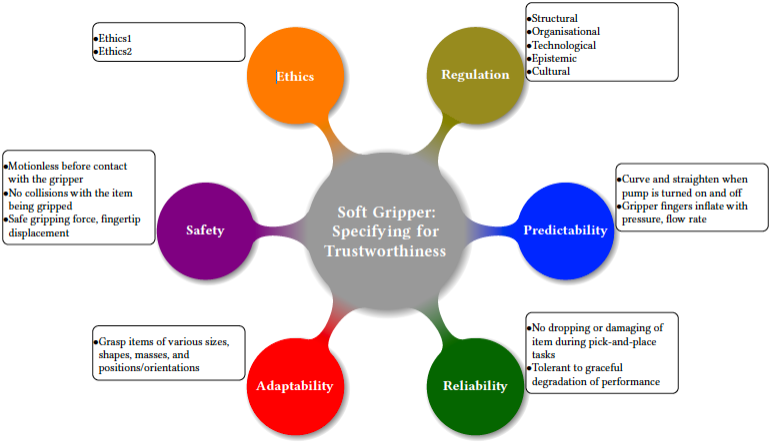
\includegraphics[width=1.0\textwidth]{figures/soft-trust.png}
	\caption{Soft gripper: Specifying for trustworthiness.}
	\label{SR-spec}
\end{figure*}

\paragraph{Predictability}\label{predictability}
Predictability is ``a property of interaction concerning the degree of confidence with which a user can determine the effect subsequent task execution will have on the achievement of the goal"~\cite{Abowd1991}. A soft gripper needs to be predictable in its behaviour, so it could build a degree of confidence and trust for end-user. 
%in the user, for instance on the expected curving of its fingers when the pump is turned on. 
%for instance changes to its curvature or finger inflation depending on other factors. %on the expected curving of its fingers when the pump is turned on.
%when its fingers curve or straighten , such as fingers need to curve when the pump is turned on.
%concerns the degree of confidence with which a user can determine the result of a future task execution will have on the achievement of a goal. 
%\emph{Predictability} centres around the future results of an interaction being determinable based on knowledge of current results.
%\emph{Predictability} concerns the ability of a system or component to perform its tasks as expected (stereotypical) without any surprises to a human. % reliably. ...
\begin{itemize}
	\item RQ1.1: The fingers of the gripper \emph{shall} curve when inflated (pump turned on).  
	\item RQ1.2: The fingers of the gripper \emph{shall} straighten when deflated (pump turned off).  
	\item RQ1.3: The curvature of a finger \emph{shall} be proportional to its internal pressure. 
	\item RQ1.4: the gripper \emph{shall} grasp, transport and place an item under same conditions with a $\ge$95\% pick-and-place repeatability.
%	\item RQ1.4: The fingers \emph{shall} be in a stable state -- pre-pressurized/inflated 10 times, prior to being used.  
	\item RQ1.5: The fingers \emph{shall} be inflated with a pressure between 3-4 psi pressure range \cite{Partridge2022}. 
	\item RQ1.6: The fingers \emph{shall} be inflated with a flow rate between 2-3.2 L/min range \cite{DEWIN2022}.
\end{itemize}

%\begin{center}
%	\begin{tabular}{|p{7mm}|p{72mm}|}
%		\hline
%		RQ1.1 & The fingers of the gripper \emph{shall} curve when inflated (pump turned on).  \\ 
%		\hline
%		RQ1.2 & The fingers of the gripper \emph{shall} straighten when deflated (pump turned off).  \\ 
%		\hline
%		RQ1.3 & The curvature of a finger \emph{shall} be proportional to its internal pressure. \\
%		\hline
%		RQ1.4 & The fingers \emph{shall} be in a stable state -- pre-pressurized/inflated 10 times, prior to being used. \\ 
%		\hline
%		RQ1.5 & The fingers \emph{shall} be inflated with a pressure between 3-4 psi pressure range. \emph{(Note: \cite{Partridge2022})} \\
%		\hline
%		RQ1.6 & The fingers \emph{shall} be inflated with a flow rate between 2-3.2 L/min range. \emph{(Note: \cite{DEWIN2022})} \\	[1ex] 		
%		\hline
%	\end{tabular}
%\end{center}

\paragraph{Reliability}\label{reliability}
\emph{Reliability} is defined as the ``ability of a system or component to perform its required functions under stated conditions for a specified period of time" \cite{ISO24765:2017}. A soft gripper needs to be reliable by not dropping or damaging items during pick-and-place tasks, and should be tolerant to graceful degradation of performance.
%\begin{center}
%	\begin{tabular}{|p{7mm}|p{72mm}|}
%		\hline
%		RQ2.1 & The gripper \emph{shall} hold the item being gripped without damaging it.  \\ 
%		\hline
%		RQ2.2 & The gripper \emph{shall} hold the item being gripped without dropping it for at least 10 seconds 95\% of the time.  \emph{(Note: \cite{Sotiropoulos2018}, pg. 652))}\\ 
%		\hline
%		RQ2.3 & The gripper \emph{shall} successfully maintain grasp during translation of the gripped item for a maximum velocity and acceleration of 0.03 m/s and 150 mm/s$^2$. \emph{(Note: \cite{Triantafyllou2019}, pg. 5; \cite{Cheng2021}, pg. 15))}\\
%		\hline
%		RQ2.4& The gripper \emph{shall} successfully grasp when the rate of inflation is in the range of 2-3.2 L/min. \emph{(Note: \cite{DEWIN2022})}\\
%		\hline
%		RQ2.5 & [\emph{Graceful degradation}] The gripper \emph{shall} experience $\le$ 5\% increase in dropping of an item across 100 hours of operation. (comment by SW: consider degradation rate instead?) \\			\hline	
%		RQ2.6 & [\emph{Graceful degradation}] The gripper \emph{shall} experience $\le$ 5\% increase in damaging of an item across 100 hours of operation.  (comment by SW: consider degradation rate instead?) \\		[1ex] 		
%		\hline
%	\end{tabular}
%\end{center}
\begin{itemize}
	\item RQ2.1: The gripper \emph{shall} hold the item being gripped without damaging it. 
	\item RQ2.2: The gripper \emph{shall} hold the item being gripped without dropping it for at least 10 seconds 95\% of the time (\cite{Sotiropoulos2018}, pg. 652).
	\item RQ2.3: The gripper \emph{shall} successfully maintain grasp during translation of the gripped item for a maximum velocity and acceleration of 0.03 m/s and 150 mm/s$^2$ (\cite{Triantafyllou2019}, pg. 5; \cite{Cheng2021}, pg. 15).
	\item RQ2.4: The gripper \emph{shall} successfully grasp when the rate of inflation is in the range of 2-3.2 L/min \cite{DEWIN2022}.
	\item RQ2.5: The gripper \emph{shall} experience $\le$ 5\% increase in dropping of an item across 100 hours of operation. %(comment by SW: consider degradation rate instead?) 
	\item RQ2.6: The gripper \emph{shall} experience $\le$ 5\% increase in damaging of an item across 100 hours of operation.  %(comment by SW: consider degradation rate instead?) 
\end{itemize}
\paragraph{Adaptability} \label{adaptability}
\emph{Adaptability} is defined as the ``degree to which a product or system can effectively and efficiently be adapted for different or evolving hardware, software or other operational or usage environments" \cite{ISO24765:2017}. In a soft gripper, \emph{adaptability} is key for manipulating objects of various sizes, shapes, masses, and positions/orientations. 
\begin{itemize}
	\item RQ3.1: The gripper \emph{shall} hold items of different sizes up to a maximum of 95\% of the opening width of the two fingers without dropping for at least 10 seconds 95\% of the time.
	\item RQ3.2: The gripper \emph{shall} hold items of different shapes (e.g. sphere, cube, cone, pyramid, cylinder) without dropping for at least 10 seconds 95\% of the time.
	\item RQ3.3: The gripper \emph{shall} hold items, which can be of regular or irregular shape, without dropping for at least 10 seconds 95\% of the time.
	\item RQ3.4: The gripper \emph{shall} hold an item independent of its orientation without dropping it for at least 10 seconds 95\% of the time. 	  
\end{itemize}
%\begin{center}
%	\begin{tabular}{|p{7mm}|p{72mm}|}
%		\hline
%RQ3.1 & The gripper \emph{shall} hold items of different sizes up to a maximum of 95\% of the opening width of the two fingers without dropping it for at least 10 seconds 95\% of the time. \\
%\hline
%RQ3.2 & The gripper \emph{shall} hold items of different shapes (e.g. sphere, cube, cone, pyramid, cylinder) without dropping it for at least 10 seconds 95\% of the time. \\[1ex] 
%\hline
%RQ3.3 & The gripper \emph{shall} hold items, which can be of regular or irregular shape, without dropping it for at least 10 seconds 95\% of the time. \\ 
%\hline
%
%
%RQ3.4 & The gripper \emph{shall} hold an item independent of its orientation without dropping it for at least 10 seconds 95\% of the time. \\ 	 
%\hline
%\emph{\sout{RQ3.5}} & \emph{\sout{Non-symmetrical objects \emph{shall} be successfully grasped (no slipping) when it is picked with X–Y* rotational offset for at least 10 seconds 95\% of the time.}}  \\ 
%\hline
%\emph{\sout{RQ3.6}} & \emph{\sout{Non-symmetrical objects \emph{shall} not be dropped when it is picked with X–Y* rotational offset for at least 10 seconds 95\% of the time.}}\\
%\hline
%\emph{\sout{RQ3.7}} & \emph{\sout{Non-symmetrical objects \emph{shall} not be damaged when it is picked with X–Y* rotational offset for at least 10 seconds 95\% of the time.}}\\
%\hline
%\emph{\sout{RQ3.8}} & \emph{\sout{For non-symmetrical objects, the grasping contact position (focus) of the gripper \emph{shall} be $\le$ X mm from the centre of the mass of the object. (Note: gripper pose agnostic, does not need to be captured).}}\\	[1ex] 
%\hline
%	\end{tabular}
%\end{center}
\paragraph{Safety}\label{safety}
\emph{Safety} is defined as an ``expectation that a system does not, under defined conditions, lead to a state in which human life, health, property, or the environment is endangered" \cite{ISO24765:2017}. 
In this study, we consider safety from the perspective of the item being gripped where physical damage should be avoided during pick-and-place tasks. % and not from any physical harm to a human.
\begin{itemize}
	\item RQ4.1: The item being gripped \emph{shall} be motionless before contact with the gripper. 
	\item RQ4.2: The gripping system \emph{shall} not collide with the item being gripped. 
	\item RQ4.3: The gripping system \emph{shall} only make contact with the item using the gripper.
	\item RQ4.4: When grasping a hard–fragile item (e.g. light bulb, raw egg), the soft actuator \emph{shall} be inflated until the gripping force does not exceed 2N (\cite{Cheng2021}, pg. 14).
	\item RQ4.5: When grasping a soft–fragile item like cake or bread, the soft actuator \emph{shall} be inflated until the fingertip displacement does not exceed 3mm (\cite{Cheng2021}, pg. 14).
	\item RQ4.6: When grasping a soft–fragile item like strawberry or bayberry, the soft actuator \emph{shall} be inflated until the gripping force does not exceed 1N and the fingertip displacement does not exceed 1mm (\cite{Cheng2021}, pg. 14).
\end{itemize}
%\begin{center}
%	\begin{tabular}{|p{7mm}|p{72mm}|}
%		\hline
%		RQ4.1 & The item being gripped \emph{shall} be motionless before contact with the gripper.   \\ 
%		\hline
%		RQ4.2 & The gripping system \emph{shall} not collide with the item being gripped. \\ 
%		\hline
%		RQ4.3 & The gripping system \emph{shall} only make contact with the item using the gripper.\\
%		\hline
%		RQ4.4 & When grasping a hard–fragile item (e.g. light bulb, raw egg), the soft actuator \emph{shall} be inflated until the gripping force does not exceed 2N. \emph{(note: \cite{Cheng2021}, pg. 14)}\\
%		\hline
%		RQ4.5 & When grasping a soft–fragile item like cake or bread, the soft actuator \emph{shall} be inflated until the fingertip displacement does not exceed 3mm. \emph{(note: \cite{Cheng2021}, pg. 14)}\\
%		\hline
%		RQ4.6 & When grasping a soft–fragile item like strawberry or bayberry, the soft actuator \emph{shall} be inflated until the gripping force does not exceed 1N and the fingertip displacement does not exceed 1mm. \emph{(note: \cite{Cheng2021}, pg. 14)}\\	[1ex] 
%		\hline
%	\end{tabular}
%\end{center}
%\clearpage
\paragraph{Ethics}\label{ethics}
\textbf{Responsible author: Arianna Manzini}\\
\textbf{(Maximum 350 words)}\\
PLACEHOLDER FOR AM\\
PLACEHOLDER FOR AM\\
PLACEHOLDER FOR AM\\
PLACEHOLDER FOR AM\\
PLACEHOLDER FOR AM\\
PLACEHOLDER FOR AM\\
PLACEHOLDER FOR AM\\
PLACEHOLDER FOR AM\\
PLACEHOLDER FOR AM\\
PLACEHOLDER FOR AM\\
PLACEHOLDER FOR AM\\
PLACEHOLDER FOR AM\\
PLACEHOLDER FOR AM\\
PLACEHOLDER FOR AM\\
PLACEHOLDER FOR AM\\
PLACEHOLDER FOR AM\\
PLACEHOLDER FOR AM\\
PLACEHOLDER FOR AM\\
PLACEHOLDER FOR AM\\
PLACEHOLDER FOR AM\\
PLACEHOLDER FOR AM\\
PLACEHOLDER FOR AM\\
PLACEHOLDER FOR AM\\
PLACEHOLDER FOR AM\\
PLACEHOLDER FOR AM\\
PLACEHOLDER FOR AM\\
PLACEHOLDER FOR AM\\
PLACEHOLDER FOR AM\\
PLACEHOLDER FOR AM\\
PLACEHOLDER FOR AM\\
PLACEHOLDER FOR AM\\
PLACEHOLDER FOR AM\\
PLACEHOLDER FOR AM\\
PLACEHOLDER FOR AM\\
PLACEHOLDER FOR AM\\
PLACEHOLDER FOR AM\\
PLACEHOLDER FOR AM\\
PLACEHOLDER FOR AM\\
PLACEHOLDER FOR AM\\
PLACEHOLDER FOR AM\\
PLACEHOLDER FOR AM\\

\paragraph{Regulation}\label{regulation}
%\textbf{Responsible author: Pete Winter}\\
%\textbf{(Maximum 350 words)}\\
Macrae’s \cite{Macrae2022} ‘SOTEC’ (structural, organisational, technological, epistemic, and cultural) framework is a useful approach for identifying domains of sociotechnical risk in autonomous and intelligent systems (AIS). The schema can help inform emergent regulation by identifying often-neglected risks. Below we outline each category and consider its application to soft gripper operations.

Structural sources of risk arise from interactions between different human and nonhuman elements in a system that amplify or transmit local failures in ways that disable the entire system. In the Soft Gripper context, for instance, such risks may arise from unanticipated disruptions, such as a human moving a grocery item, confusing the perception system. Regulatory requirements should ensure the system anticipates and accommodates the complexities of human-machine interactions.

Organisational sources of risk emerge when organisational structures, such as rules and expectations, are insensitive to the vagaries of real human behaviour. For example, protocols for checking the soft gripper might presuppose an unrealistic degree of diligence. Regulatory requirements should be alert to the practical dimensions of potential rules and procedures.

Technological sources of risk arise from shortcomings of the system itself. These are the myriad risks that engineers would conventionally consider as part of their work. In the context of soft-grippers, for example, there is concern about elastomers degrading and shedding material into food. Regulators should ensure that designers effectively test properties, limits and behaviours.

Epistemic sources of risk arise from the inherent indeterminacies of knowledge, which create pockets of ignorance that hide unexpected hazards. Such pockets are difficult to mitigate (since we don’t know what we don’t know) but it can be anticipated that soft grippers could fail for unexpected reasons, and tailor regulatory provisions in ways that promote resilience and learning. 

Cultural sources of risk arise from collective values — beliefs, norms, mores — that frame and influence AIS design and operation. So it might be, for instance, that grippers might come to be optimised for overall efficiency even if it means they underperform in niche tasks that only affect a minority of stakeholders. Regulatory requirements must reflect critically on their underlying values, and work to counter potential inequities. 

%PLACEHOLDER FOR PW\\
%PLACEHOLDER FOR PW\\
%PLACEHOLDER FOR PW\\
%PLACEHOLDER FOR PW\\
%PLACEHOLDER FOR PW\\
%PLACEHOLDER FOR PW\\
%PLACEHOLDER FOR PW\\
%PLACEHOLDER FOR PW\\
%PLACEHOLDER FOR PW\\
%PLACEHOLDER FOR PW\\
%PLACEHOLDER FOR PW\\
%PLACEHOLDER FOR PW\\
%PLACEHOLDER FOR PW\\
%PLACEHOLDER FOR PW\\
%PLACEHOLDER FOR PW\\
%PLACEHOLDER FOR PW\\
%PLACEHOLDER FOR PW\\
%PLACEHOLDER FOR PW\\
%PLACEHOLDER FOR PW\\
%PLACEHOLDER FOR PW\\
%PLACEHOLDER FOR PW\\
%PLACEHOLDER FOR PW\\
%PLACEHOLDER FOR PW\\
%PLACEHOLDER FOR PW\\
%PLACEHOLDER FOR PW\\
%PLACEHOLDER FOR PW\\
%PLACEHOLDER FOR PW\\
%PLACEHOLDER FOR PW\\
%PLACEHOLDER FOR PW\\
%PLACEHOLDER FOR PW\\
%PLACEHOLDER FOR PW\\
%PLACEHOLDER FOR PW\\
%PLACEHOLDER FOR PW\\
%PLACEHOLDER FOR PW\\
%PLACEHOLDER FOR PW\\
%PLACEHOLDER FOR PW\\
%PLACEHOLDER FOR PW\\
%PLACEHOLDER FOR PW\\
%PLACEHOLDER FOR PW\\
%PLACEHOLDER FOR PW\\
%PLACEHOLDER FOR PW\\

\section{Verifiability of a Soft Gripper} \label{verifiability}
%6.2 Verification and validation methodsVerification and validation can be satisfied by methods including but not limited to:—A visual inspection;—B practical tests;—C measurement;—D observation during operation;—E review of application-specific schematics, circuit diagrams and design material;—F review of safety-related application software and/or software documentation;—G review of task-based risk assessment;—H review of layout drawings and documents;—I review of specifications and information for use.See Table G.1.


The notion of \emph{verifiability} is considered key for improving trustworthiness of an AS, such as a soft robotic system. 
A unified and holistic approach to verifiability will fundamentally change the approach to verifying ASs, which will lead to systems that are by their construction worthy of our trust \cite{Mousavi2022}. 
%Our vision is that such a unified andholistic approach to verifiability will fundamentallychange our approach to the verification ofautonomous systems and will lead to systems thatare by their construction are worthy of our trust.
%To this end, one can seek to promote verifiability to a first-class system design objective \cite{Eder2021}. ...
Verifiability can be achieved by considering verification early, such as during specification and system design \cite{Mousavi2022} where it can be promoted to a first-class system design objective \cite{Eder2021}. 

For a system to be {\em verifiable\/}, a person or a tool needs to be able to check its correctness~\cite{ISO24765:2017} with respect to its requirements and specification \cite{Abeywickrama2022}. 
The main challenge is in specifying and designing the system in such a way that this process is made as easy and intuitive as possible.
%
For ASs in particular, specific challenges include 
%
(i) capturing and formalizing requirements including functionality, safety, security, performance and, beyond these, any additional non-functional requirements purely needed to demonstrate trustworthiness; 
%	 
(ii) handling flexibility, adaptation and learning; and 
%
(iii) managing the inherent complexity and heterogeneity of both the AS and the environment it operates in. 
%With respect to these i--iii challenges, our study has taken key steps towards addressing them. We propose a wide-ranging specification of requirements to demonstrate trustworthiness (Section~\ref{specification-gripper}); and the specification includes requirements that adapts the soft gripper to objects of different sizes, shapes, masses and orientations/positions.


Gerson~\cite{Gerson1993} identifies several techniques for ensuring verifiability: bounding the verification task, prioritizing effort, ensuring traceability, and breaking down high-level requirements into verifiable portions. 
According to Gerson, formulating requirements for verifiability should go far beyond avoiding negative requirements and including numerical tolerances, but also aim to \emph{design for verifiability}. 
This is because the ultimate purpose of specifications is verifying that the end product exhibits the intended properties. 
This requires the intended properties to be \emph{demonstrable}, that is knowledge of the end result needs to be attainable. 
In our study, we have considered this early when formulating requirements, by planning and confirming how these properties can be verified later (see Table~\ref{Table:Verifiability}). 

For example, requirements 1.1, 1.2, 1.4, 2.1, 2.2 and 2.4 can be verified by \emph{observing} the gripping system during operation. 
Observation is ``a technique that provides a direct way of viewing individuals in their environment performing their jobs or tasks and carrying out processes"~\cite{ISO24765:2017}.
Let us describe a unit test that can be conducted to verify requirement RQ1.5. 
A two-fingered soft pneumatic gripper can be fabricated as proposed in \cite{Partridge2022} using 30\% recycled material. 
One can use black pigments to track the chambers and granules, and red pigments to track the curvature of the constraining layer. 
Then the fingers can be actuated and their motion can be captured with a camera. 
Curvature with time can be determined by conducting image processing on the video. Also, internal pressure with time can be monitored.

% Re robot paper
%The fingers can be removed and replaced independently,facilitating in-factory replacement, recycling and reuse. Thefingers are pneumatically actuated to grip a range of objectsincluding a Rubik’s cube, a small rubber duck, a sponge balland a fresh egg.Two fingers were fabricated, one with pristine silicone andthe other with 30\% 1 to 2 mm granules, for comparison. Ablack pigment was used for the chambers and granules andred pigment for the constraining layers to allow curvatureof the constraining layer to be tracked. The fingers werethen actuated and their motion was captured with a camera.Image processing was then conducted on the video such thatcurvature with time could be determined. Internal pressurewith time was also monitored.
%
%For example, 
%For the gripper testing (see Figure 7), the pressure responsein each finger is almost equal. However, the recycledfinger is only able to achieve 80% of the effective curvatureachieved by the pristine finger. As with the pneumatic actuator,this means that increased pressure will be required toachieve the same curvature as the pristine finger. This is stillsufficient for gripping purposes, but should be consideredwhen utilising recycled actuators in gripping systems.



%Following this guidance, let us examine how our specification meets it.

%IV. EXPERIMENTAL METHODS FOR BUCKLINGANALYSISA. Pressure and Volume To test the pressure response with volume for each configuration of buckling element (regular, fully constrained and offset), each pneu-net was loosely fitted to a black acrylicstand, such that they lay flat when unactuated but were notobstructed. Each configuration was then placed against ablack background and again attached to a pressure sensor.The pressure sensor was positioned as close to the base ofthe pneu-net as possible without interfering with the imagedata (roughly 2cm from the base) and connected to a syringe.The syringe was set at 30ml of volume and lay within a linearactuator that acted on the base to actuate the pneu-nets. Alaser distance sensor (LK-G152, Keyence) was set to measurethe displacement of the end of the syringe as it moved,thus allowing for an accurate volume measurement withtime. Both the pressure and laser distance sensor attachedto a DAQ (USB-6001 Multifunction I/O Device, NationalInstruments). Data was collected and processed in MatLab(Figure 5). The pressure / volume data allows comparisonsto be drawn between the pneu-nets and to examine how theaddition of buckling elements affects the pressure requiredto achieve actuation.
%Fig. 5. Test set up for pressure and volume data acquisition. i) The syringeconnected to a linear actuator rail. ii) NI DAQ. iii) Pressure sensor. iv) Pneunetwith buckling element. v) LED to synchronise video data with DAQ data.vi) Linear actuator switch. vii) Laser distance sensor behind black screen.


%According to Gerson~\cite{Gerson1993}, system engineers need to design the system for \emph{verifiability}, as the ultimate purpose of specifications is verifying that the end product exhibits the intended properties. 
%This requires the intended properties to be \emph{demonstrable}, i.e. that knowledge of the end result needs to be attainable. 
%In our study, we have considered this early during specification, by confirming how these properties can be verified later (see Table~\ref{Table:Verifiability}). For example, requirements 1.1, 1.2, 1.4, 2.1, 2.2 and 2.4 can be verified by observing the gripping system during operation. GIVE EXAMPLE...

Following the guidance provided in \cite{NASA2007} on how to write good requirements, engineering requirements in Section~\ref{specification-gripper} have been formulated positively (i.e. use of \emph{shall} statements as opposed to \emph{shall not} statements). 
In addition, most requirements of the specification contain numeric tolerances. 
Still, there are several high-level requirements in the specification, which need to be refined into verifiable portions before any verification method can be applied. % this is the original one. 1.1 as it is it cannot be verified so we can use this as an example. how to make it verifiable? this is a refined version of this step. it is verifiable because we have now instantiated it.  
For instance, requirements RQ1.1--1.3 have been formulated in a high-level because the amount of curvature and straightening of a finger can often be dependent on the application. 
In order to be verifiable, we can refine RQ1.1 as: the fingers of the gripper \textit{shall} curve within 2\% of summed difference between a curve of 10 cm radius when inflated. 
Similarly, we can breakdown other high-level requirements of the specification such as RQ4.1--4.3. ...
%Requirement RQ4.1 can be verified using a vision camera to inspect whether the item is moving or not. 
%RQ4.2 can be verified using a force torque sensor, and 4.3 can be verified using both force torque sensor and vision camera. 
%summed difference score is the sum of the differences between the stress and rest scores 

On the other hand, requirements like RQ1.5 have identified a specific range of tolerance values (e.g. pressure range). % that is the right way of doing. 
Similarly, in RQ4.4, we identify a maximum bound value of 2N for gripping force when gripping a hard-fragile item. 
Therefore, our study provides two versions of the specification -- one a \emph{verifiable} one from the start, and the other a more \emph{high-level} one, for which we using examples show how to make it verifiable. 
By doing this, we show what is the difference or delta between a high-level requirement and its verifiable version. 
In this manner, our study not only provides a wide-ranging specification for a pick-and-place application, but it also goes a step further by providing design guidelines towards the formulation of verifiable requirements for the soft robotics community. % requirements verifiable.

%And identify already that they need to be parameters and and that's the right way of doing this. So if we if we leave it like this as the raw set of requirements and it says. 
%I see two versions I see the version of the paper where we consider verifiability from the start and we give them what we consider the verifiable version and we then argue why this is verifiable on some selected examples or we do the raw requirements as they are now and then in the verifiability section we say well.
%For verifiability is very important to have these parameters and to to to to understand what they mean, what the Rangers are, etcetera.
%And let's look at uh 1.1 this as it is in its raw state is not verifiable because and here is the verifiable version.
%Umm. And that is verifiable because and so we could possibly with the 2nd way of doing this, make a much stronger point so that people see what the delta is between the raw and the what we consider verifiable.



%Through this we provide guidelines to the soft robotics community on how to make requirements 
%
%
%
%There are some requirements in the specification where we consider verifiability from the start. 
%We can argue why these set of requirements are verifiable. 
%This instantiation of the generic requirement is very much needed to support its verifiability. 
%
%
%
%
%the amount of curvature expected in mm or as a percentage of the diameter. 
%Similarly, RQ1.2 can mention how much degrees a finger needs to straighten when the pump is turned off. 


\begin{table}[!t]
	\centering
	\begin{tabular}{|p{32mm}|p{50mm}|}
		\hline
		\textbf{Requirements} & \textbf{Verification Method} \\ 
		\hline
		RQ1.1, 1.2, 1.4, 2.1, 2.2, 2.4 & Observation during operation\\%Visual Inspection \\
		\hline
		RQ1.3, 1.5 & Practical tests: unit testing  \\
		\hline
		RQ2.3 & Practical tests: edge-case Testing \\
		\hline
		RQ2.5, 2.6 & Practical tests: life-cycle testing \\
		\hline
		RQ3.1, 3.2, 3.3 & Practical tests: repeated testing and Observation \\
		\hline
		RQ4.1 & Measurement: vision camera, observation  \\ 
		\hline
		RQ4.2 & Measurement: force torque sensor \\ 
		\hline
		RQ4.3 & Measurement: force torque sensor and vision camera  \\ 
		\hline
		RQ4.4 & Practical tests: functional test\\ 
		\hline
		RQ4.5 & Measurement: displacement sensor   \\ 
		\hline
		RQ4.6 & Both Practical tests and Measurement (functional test and displacement sensor) \\ 
		\hline
	\end{tabular}
	\caption{\label{Table:Verifiability} Soft-gripper requirements and verification methods.}
\end{table}
%RQ4.1 & you can build this by vision camera to check whether it is moving or not, or just inspect. but a motion, camera will tell you exactly, so it'll be mounted one on somewhere, either on robot arm and effects or whatever. I'll be able to tell you, or just just outside it within the robot workspace, mounting it somewhere.. even inspection is Ok.  \\ 
%RQ4.2 & More like, you know, tactile sensor, force torque sensor reading. Because this comes back to it not being damaged, the item right, so it has to be appropriate force being applied. So you can build that into your force torque sensor. This sensor is used -, the forced to see whether it's colliding with the item, right. \\ 
%RQ4.3 & The gripping system shall only made contact with the item using the gripper. Yeah, that's basically comes down to, you know, the force torque sensor or the load cell being applied on the gripper and on the rest of the arm. Just check that. So tactile sensing will tell you these information. force torque sensor and vision (camera). Put together. \\ 


%While most requirements in the specification are {\em verifiable\/}, still some requirements are abstract in nature. 
%For example, ....

%Discuss how the requirements in the specification can be made verifiable. Discuss raw requirements... verifiable version and the delta...
%Usability and Verifiability of Secure Features for Authenticating Identity
%Verifiability differs from verification that in verifiability it is unknown at the start what is the level of verification can be done to the feature.
%
%
%Verifiability differs from verification that in verifiability it is unknown at the start
%what is the level of verification can be done to the feature.
%
%Verification should be raised to a design concern, which is what verifiability is about. 
%So do not state requirements that you don't know how to verify the moment state to requirement. You need to confirm how you would verify it.
%And if you can't do that, it's not worth it.
%
%the generic version, and then the instantiation...
%
%How do you make this verifiable? Well, in order to make it verifiable, we need to know these things, and here is a refined version of this step we can deem verifiable because we've now instantiated it. But look at 1.5 and 1.5 in the original requirements.
%
%Raw version.. verifiable version...
%delta for 
%
%what a proper  curve shall be or what is straightness
%
%to make a verifiable spec what needs to do
%
%visible the delta... raw sets of reqts.. purpose of this section.. skim them how would i do it... KE
%what are the techniques 
%process should go through
%
%change between the original raw instantiation of raw specification
%designer, req eng... question is how do you verify it
%designer might come up with an idea
%
%what the delta is between the raw and the what we consider verifiable
%
%purpose of this section is to highlight that that's not enough to to make verifiability
%\begin{center}
%	\begin{tabular}{|p{15mm}|p{50mm}|}
%			\hline
%			\textbf{Reqt.} & \textbf{Verification technique} \\ 
%			\hline
%			RQ1.1 & Just a test. visual inspection. if finger does not curve there is leakage...  \\ 
%			\hline
%			RQ1.2 & Just a test. visual inspection.  \\ 
%			\hline
%			RQ1.3 & Unite test (test one finger in paper...fig 7 thats what the unit test we do...performance unit testing).  \\ 
%			\hline
%			RQ1.4 & Subjective. it is better if we follow a specific equation first. better to cite a paper.. have not seen exactly. if this is just for recycled soft gripper i will check alex paper.. 5 to 10 inflatable cycles.. alex has a paper. may be you can reference alex paper - he has a paper...tries to find.. verification tech - unit test to check the (11:20 said will send it) \\ 
%			\hline
%			RQ1.5 & test in the paper. optimal pressure range fingers would curve into desired curvature. Block test. Or call it a unit test.. hang on isometric test is testing the strength.. don't use that term. just use unit test or block test... Figure 7a..  \\ 
%			\hline
%			RQ1.6 & just pump operational range. no test we just follow the specification of the pump...and pump will not work beyond... pump manufacturer would already verified that   \\ 
%			\hline
%			RQ2.1 & Inspection as well.  \\ 
%			\hline
%			RQ2.2 & Visually inspecting. Inspect as well. data recording and repeated test  \\ 
%			\hline
%			RQ2.3 & Testing and trying errors. You have upper bound. you try upper bound and see if it works. Verification - Edge cases test (extreme test). It is still operational under extreme cases. step it up until max value and outside that value it does not work as expected. out of bound. checking upper bound and lower bound and edge cases. doing tests...  \\ 
%			\hline
%			RQ2.4 & Inspection, you see if it grasp the object or not.  \\ 
%			\hline
%			RQ2.5 & Material dependent (silicon). Doing in cycle. what is the degradation rate you expect. relates to 95\% one. if it is less than 95 it become unsuable. that is what you have to test for. .from same test measure data (degradation of performance... benchmark.. deviate .. don't work .. affect successful operation. need to replace it)  And later say for example is like. Basically you can see the decoration of the performance, meaning that it doesn't really perform. So for example, you've got a benchmark of. It's always curve, not much when the pressure pumped it is this X amount, right? But then as it degrades, not gonna curve that exactly like that anymore, but it would deviate from that. It's either more or less. So if it deviate.
%			Uh. Outside a certain range, it doesn't work at expected anymore and that then we will say and then at that number will affect the successful right of operation a bit as well.
%			And that if it fall out of that range, then you say, yeah, it's it's not usable anymore. You need to replace it. ... correct - if you cant grasp and drops in 10 sec it is not a functional gripper anymore
%			\\ 
%			\hline
%			RQ2.6 &   \\ 
%			\hline
%			RQ3.1 & long term repeating test. traditional one.. inspection observation .. may be graham might know. life span of a piece of equipment. life span test. it is a test. manufacturer do. LIFE CYCLE TESTING... this could be for degradation. for this variety testing of different categories. physical testing, observing and recording - dhaminda.  \\ 
%			\hline
%			RQ3.2 & Inspection.  \\ 
%			\hline
%			RQ3.3 & ... same as 3.1 repeated variety test as well. also 3.4  \\ 
%			\hline
%			RQ4.1 & you can build this by vision camera to check whether it is moving or not, or just inspect. but a motion, camera will tell you exactly, so it'll be mounted one on somewhere, either on robot arm and effects or whatever. I'll be able to tell you, or just just outside it within the robot workspace, mounting it somewhere.. even inspection is Ok.  \\ 
%			\hline
%			RQ4.2 & More like, you know, tactile sensor, force torque sensor reading. Because this comes back to it not being damaged, the item right, so it has to be appropriate force being applied. So you can build that into your force torque sensor. This sensor is used -, the forced to see whether it's colliding with the item, right. \\ 
%			\hline
%			RQ4.3 & The gripping system shall only made contact with the item using the gripper. Yeah, that's basically comes down to, you know, the force torque sensor or the load cell being applied on the gripper and on the rest of the arm. Just check that. So tactile sensing will tell you these information. force torque sensor and vision (camera). Put together. \\ 
%			\hline
%			RQ4.4 & capability test or functional test (functional test - functional test is basically testing whether is perform a specific function). Measure in Newtons - could use load cell for this on to the gripper and  then basically  just keep inflating the gripper until you crossed it and then that's the force.. keep increasing the force until it reached like a critical Max force that break the thing. Uh, we call it test to failure, but then when it breaks and you know that you can't accept that. Test to failure: it is normally they  do it in tensile testing when it stretch a piece of material or they pull a piece of material until it breaks and that will be the the maximal, the maximum force that piece of material can take. This is not a Tensile test but it is a function test. But it has the same principle. 
%			 \\ 
%			\hline
%			RQ4.5 & fingertip displacement - proximity sensor.It's sort of like measuring like the deviation distance...correct -- displacement sensor would tell you one thing has displaced. So displacement sensor will tell you how much.
%			One thing's been displaced by   \\ 
%			\hline
%			RQ4.5 & both sensor -- either displacement sensor, vission camera. Yeah. And then you either displacement sensor, you can use vision camera also tell you this as well so. Yeah, but but then you don't want to over. Uh, complicated your system so displacement sensor would. Brought out of finger tape will tell you this information. \\ \hline
%		\end{tabular}
%\end{center}


%pressure and volume 4a) unit test or functional test- this is how you would do that. this one is a different functional test ..38:00 process is same. 1.5, 1.6... test setup is very similar to 

%Meanwhile, \emph{verifiability} is considered key for improving trustworthiness, which can be realized by considering verification early as an integral part during specification, and system design \cite{Mousavi2022} where it can be promoted to a first-class system design objective \cite{Eder2021}. 
%Verifiability will essentially lead to systems that are by their construction are worthy of our trust. 
%PLACEHOLDER FOR VERIFIABILITY \\
%PLACEHOLDER FOR VERIFIABILITY \\
%PLACEHOLDER FOR VERIFIABILITY \\
%PLACEHOLDER FOR VERIFIABILITY \\
%PLACEHOLDER FOR VERIFIABILITY \\
%PLACEHOLDER FOR VERIFIABILITY \\
%PLACEHOLDER FOR VERIFIABILITY \\
%PLACEHOLDER FOR VERIFIABILITY \\
%PLACEHOLDER FOR VERIFIABILITY \\
%PLACEHOLDER FOR VERIFIABILITY \\
%PLACEHOLDER FOR VERIFIABILITY \\
%PLACEHOLDER FOR VERIFIABILITY \\
%PLACEHOLDER FOR VERIFIABILITY \\
%PLACEHOLDER FOR VERIFIABILITY \\
%PLACEHOLDER FOR VERIFIABILITY \\
%PLACEHOLDER FOR VERIFIABILITY \\
%PLACEHOLDER FOR VERIFIABILITY \\
%PLACEHOLDER FOR VERIFIABILITY \\
%PLACEHOLDER FOR VERIFIABILITY \\
%PLACEHOLDER FOR VERIFIABILITY \\
%PLACEHOLDER FOR VERIFIABILITY \\
%PLACEHOLDER FOR VERIFIABILITY \\
%PLACEHOLDER FOR VERIFIABILITY \\
%PLACEHOLDER FOR VERIFIABILITY \\

%In this subsection, we will discuss how we propose to make the requirements verifiable (raw requirements to verifiable requirements, and explain the delta)...

%are both functional and non-functional (thus, supporting i), and the adaptability requirements support ii
%In the previous subsection, we provided a set of functional and non-functional requirements 

%Specifications need to represent the different aspects of the overall system in a way that is natural to domain experts, facilitates modelling and analysis, provides transparency of how the AS works and gives insights into the reasons that motivate its decisions. 
%%
%To specify for verifiability, a specification framework will need to offer a variety of domain abstractions to represent the diverse, flexible and possibly evolving requirements ASs are expected to satisfy. 
%%
%Furthermore, the underlying verification framework should connect all these domain abstractions to allow an analysis of their interaction. This is a key challenge in specification for verifiability in ASs.
%
%\begin{itemize}
%	\item Describe above in the context of a soft gripper – how we can consider above i––iii when specifying for trustworthiness for a soft gripper.
%	\item Also, how we can provide for domain abstractions...
%\end{itemize}
%...\\





%\cite{Cheng2021,Bhattacharya2019,Bianchi2018,Cai2021,Chen2018,Hong2022,Farrell2022,Hwang2020,Liu2021,Loh2014,Mohan2020,Negrello2020,Nishikawa2019,Pozzi2016,Shin2021,Sotiropoulos2018,Tadakuma2020,Triantafyllou2019}

\section{Summary and Conclusions} \label{summary-conclusions}
\noindent PLACEHOLDER FOR SUMMARY AND CONCLUSIONS\\
PLACEHOLDER FOR SUMMARY AND CONCLUSIONS\\
PLACEHOLDER FOR SUMMARY AND CONCLUSIONS\\
PLACEHOLDER FOR SUMMARY AND CONCLUSIONS\\
PLACEHOLDER FOR SUMMARY AND CONCLUSIONS\\
PLACEHOLDER FOR SUMMARY AND CONCLUSIONS\\
PLACEHOLDER FOR SUMMARY AND CONCLUSIONS\\
PLACEHOLDER FOR SUMMARY AND CONCLUSIONS\\
PLACEHOLDER FOR SUMMARY AND CONCLUSIONS\\
PLACEHOLDER FOR SUMMARY AND CONCLUSIONS\\
PLACEHOLDER FOR SUMMARY AND CONCLUSIONS\\
PLACEHOLDER FOR SUMMARY AND CONCLUSIONS\\
PLACEHOLDER FOR SUMMARY AND CONCLUSIONS\\
PLACEHOLDER FOR SUMMARY AND CONCLUSIONS\\
PLACEHOLDER FOR SUMMARY AND CONCLUSIONS\\
PLACEHOLDER FOR SUMMARY AND CONCLUSIONS\\
PLACEHOLDER FOR SUMMARY AND CONCLUSIONS\\
PLACEHOLDER FOR SUMMARY AND CONCLUSIONS\\
PLACEHOLDER FOR SUMMARY AND CONCLUSIONS\\
PLACEHOLDER FOR SUMMARY AND CONCLUSIONS\\
PLACEHOLDER FOR SUMMARY AND CONCLUSIONS\\
PLACEHOLDER FOR SUMMARY AND CONCLUSIONS\\
PLACEHOLDER FOR SUMMARY AND CONCLUSIONS\\
PLACEHOLDER FOR SUMMARY AND CONCLUSIONS\\
PLACEHOLDER FOR SUMMARY AND CONCLUSIONS\\
PLACEHOLDER FOR SUMMARY AND CONCLUSIONS\\
PLACEHOLDER FOR SUMMARY AND CONCLUSIONS\\
PLACEHOLDER FOR SUMMARY AND CONCLUSIONS\\
PLACEHOLDER FOR SUMMARY AND CONCLUSIONS\\
PLACEHOLDER FOR SUMMARY AND CONCLUSIONS\\
PLACEHOLDER FOR SUMMARY AND CONCLUSIONS\\
PLACEHOLDER FOR SUMMARY AND CONCLUSIONS\\
PLACEHOLDER FOR SUMMARY AND CONCLUSIONS\\
PLACEHOLDER FOR SUMMARY AND CONCLUSIONS\\
PLACEHOLDER FOR SUMMARY AND CONCLUSIONS\\
PLACEHOLDER FOR SUMMARY AND CONCLUSIONS\\
PLACEHOLDER FOR SUMMARY AND CONCLUSIONS\\
PLACEHOLDER FOR SUMMARY AND CONCLUSIONS\\
PLACEHOLDER FOR SUMMARY AND CONCLUSIONS\\
PLACEHOLDER FOR SUMMARY AND CONCLUSIONS\\


\section*{Acknowledgments}
The work presented in this paper has been supported by the UK Engineering and Physical Sciences Research Council (EPSRC) under the grant [EP/V026518/1].

\bibliographystyle{IEEEtran}
\bibliography{Spec-SoftRobotics-Bibliography.bib}

\newpage

\vfill

\end{document}